\section{Apresentação do Trabalho}
\label{sec:apresentacao}


\section{Introdução}
Este trabalho tem como objetivo a análise da envoltória do momento fletor em uma viga isostática sob a ação de uma carga móvel. O estudo inclui a consideração de cargas permanentes e móveis e a determinação dos valores máximos e mínimos do momento fletor ao longo da viga.


\section{Dados para o Trabalho}
Os seguintes valores devem ser adotados:
\begin{table}[h]
    \centering
    \begin{tabular}{|c|c|c|c|c|c|c|}
        \toprule \hline
        \textbf{Equipe} & $c$ (m) & $b$ (cm) & $h$ (cm) & $F_1=F_2$ (kN) & $F_3$ (kN) & $q_{\text{móvel}}$ (kN/m) \\  \hline
        \midrule  \hline
        01              & 2,0     & 30       & 100      & 4,0            & 12,0       & 2,0                       \\  \hline
        \bottomrule
    \end{tabular}
    \caption{Parâmetros para o cálculo da envoltória}
    \label{tab:parametros}
\end{table}


\section{Definições e Parâmetros}

\subsection{Viga Isostática sob a Ação de uma Carga Móvel}
A viga isostática será submetida a um carregamento móvel do tipo trem, além de sua carga permanente correspondente ao peso próprio do concreto armado e de esforços pontuais.

\subsection{Carga Permanente}
A carga permanente é representada pelo peso próprio da viga, considerando uma seção de dimensões $b \times h$ cm$^2$:

\begin{itemize}
    \item base da viga: $b=30cm$ cm;
    \item altura da viga: $h=100cm$ cm.
    \item densidade específica do concreto: $\rho=2000 kg/m^3$
    \item aceleração da gravidade: $g=9,81 m/s^2$
    \item carga permanente: $q_{\text{perm}} = \rho \cdot g \cdot b \cdot h = 5,886 kN/m$ \textdownarrow
    \item Módulo de Elasticidade do Concreto: $E_c = 200 GPa$
    \item Inércia da Seção Transversal: $I = \frac{b \cdot h^3}{12} \rightarrow I = 2.5 \times 10^6 \text{ cm}^4$
    \item Distância entre as forças: $d = 1,5 m$
    \item Comprimento de secção: $c = 2 m$
    \item Número de seções: $n = 11$ (incluindo as extremidades)
\end{itemize}

\begin{figure}[h]
    \centering
    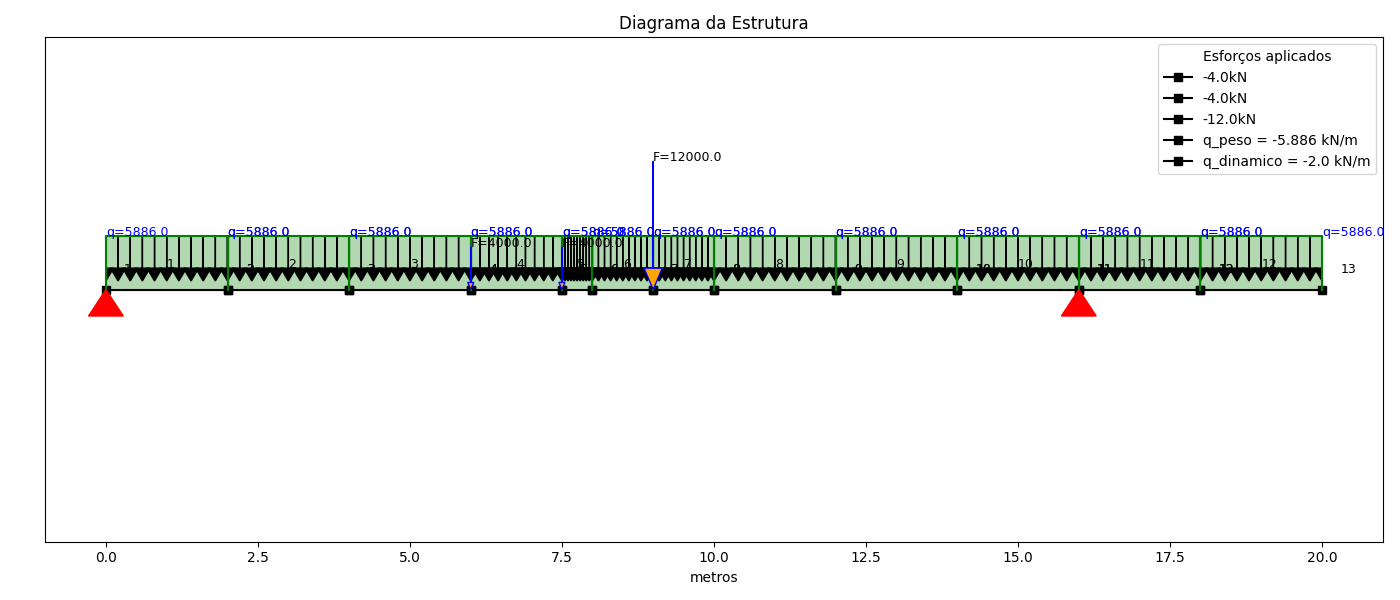
\includegraphics[width=1\linewidth]{images/diagrama}
    \caption{Viga Isostática Simulada}
    \label{fig:viga_isostatica}
\end{figure}

\subsection{Cargas Móveis}
O carregamento móvel é representado por um trem-tipo, com as seguintes características:
\begin{itemize}
    \item carga móvel: $q_{\text{móvel}} = 2 kN/m$ \textdownarrow
    \item Forças pontuais: $F_1 = F_2 = 4 kN$ e $F_3 = 12 kN$ \textdownarrow
    \item comprimento do trem: $L = 1.5 m$
    \item distância entre os trens: $a = 0 m$
    \item número de trens: $n = 3$
\end{itemize}

As três cargas móveis foram distrubidas entre os pontos \textit{S4} e \textit{S6} da viga. Além dos carregamentos pontuais $F_1$, $F_2$ e $F_3$. que também foram distribuídos entre os mesmos pontos.


\section{Memorial de Cálculo}
A viga será dividida em 11 seções, incluindo as extremidades. O cálculo do momento fletor será realizado para cada seção, considerando a carga permanente e móvel. O momento fletor será calculado para as seguintes situações:
O Cálculo se inicia com a identificação dos esforços cortantes e das reações de apoio. A partir daí, é possível determinar o momento fletor em cada seção da viga.

\begin{equation}
    \sum F_y = 0 \Rightarrow R_A + R_B = q_1 \cdot 20 + q_2 \cdot 4 + (P_1 + P_2 + P_3)
\end{equation}

\begin{equation}
    \sum M_A = 0 \Rightarrow R_B \cdot 16 - q_1 \cdot 20 \cdot \frac{20}{2} - q_2 \cdot 4 \cdot \left(\frac{6+10}{2}\right) - P_1 \cdot 6 - P_2 \cdot 7.5 - P_3 \cdot 9 = 0
\end{equation}


\section{Tabela de Cálculo da Envoltória}
A envoltória do momento fletor deve ser calculada conforme a tabela a seguir:
\begin{table}[h]
    \centering
    \begin{tabular}{|c|c|c|c|c|c|}
        \toprule \hline
        \textbf{Seção} & $M_{\text{perm}}$ (kN.m) & $M_{\text{móvel,max}}$ (kN.m) & $M_{\text{móvel,min}}$ (kN.m) & $M_{\text{max}}$ (kN.m) & $M_{\text{min}}$ (kN.m) \\
        \midrule  \hline
        S1             & 0                        & 0                             & 0                             & 0                       & 0                       \\ \hline
        S2             &                          &                               &                               &                         &                         \\ \hline
        S3             &                          &                               &                               &                         &                         \\ \hline
        S4             &                          &                               &                               &                         &                         \\ \hline
        S5             &                          &                               &                               &                         &                         \\ \hline
        S6             &                          &                               &                               &                         &                         \\ \hline
        S7             &                          &                               &                               &                         &                         \\ \hline
        S8             &                          &                               &                               &                         &                         \\ \hline
        S9             &                          &                               &                               &                         &                         \\ \hline
        S10            &                          &                               &                               &                         &                         \\ \hline
        S11            & 0                        & 0                             & 0                             & 0                       & 0                       \\  \hline
        \bottomrule
    \end{tabular}
    \caption{Tabela para o traçado da envoltória}
    \label{tab:envoltoria}
\end{table}


\section{Gráficos da Envoltória}
Para a construção da envoltória, serão traçadas três curvas:
\begin{itemize}
    \item \textbf{Curva 1 (preta)}: Representa os valores da coluna (1) da Tabela \ref{tab:envoltoria}.
    \item \textbf{Curva 2 (vermelha)}: Representa os valores da coluna (4).
    \item \textbf{Curva 3 (azul)}: Representa os valores da coluna (5).
\end{itemize}


\section{Conclusão}
Os resultados obtidos devem ser analisados e discutidos, levando em consideração os efeitos da carga móvel e permanente sobre o comportamento estrutural da viga.


\section{Observações}
\begin{enumerate}
    \item O trabalho deve ser entregue em sala no dia XX/02/25 (terça-feira).
    \item A equipe deve conter até quatro participantes.
    \item Os cálculos devem ser apresentados manuscritos.
    \item Os gráficos devem ser gerados em software gráfico.
    \item O coordenador deve anexar a lista dos participantes e suas respectivas tarefas.
\end{enumerate}


\section{Referências Bibliográficas}
\begin{itemize}
    \item ALMEIDA, Maria Cascão Ferreira de. \textit{Estruturas Isostáticas}. Carga Móvel (Páginas 143 a 164).
\end{itemize}